\section{ATLAS}

, \cite{collaboration_2020}, \cite{Owen:2302730} 






\subsection*{Data collection}

\begin{figure}[h!]
    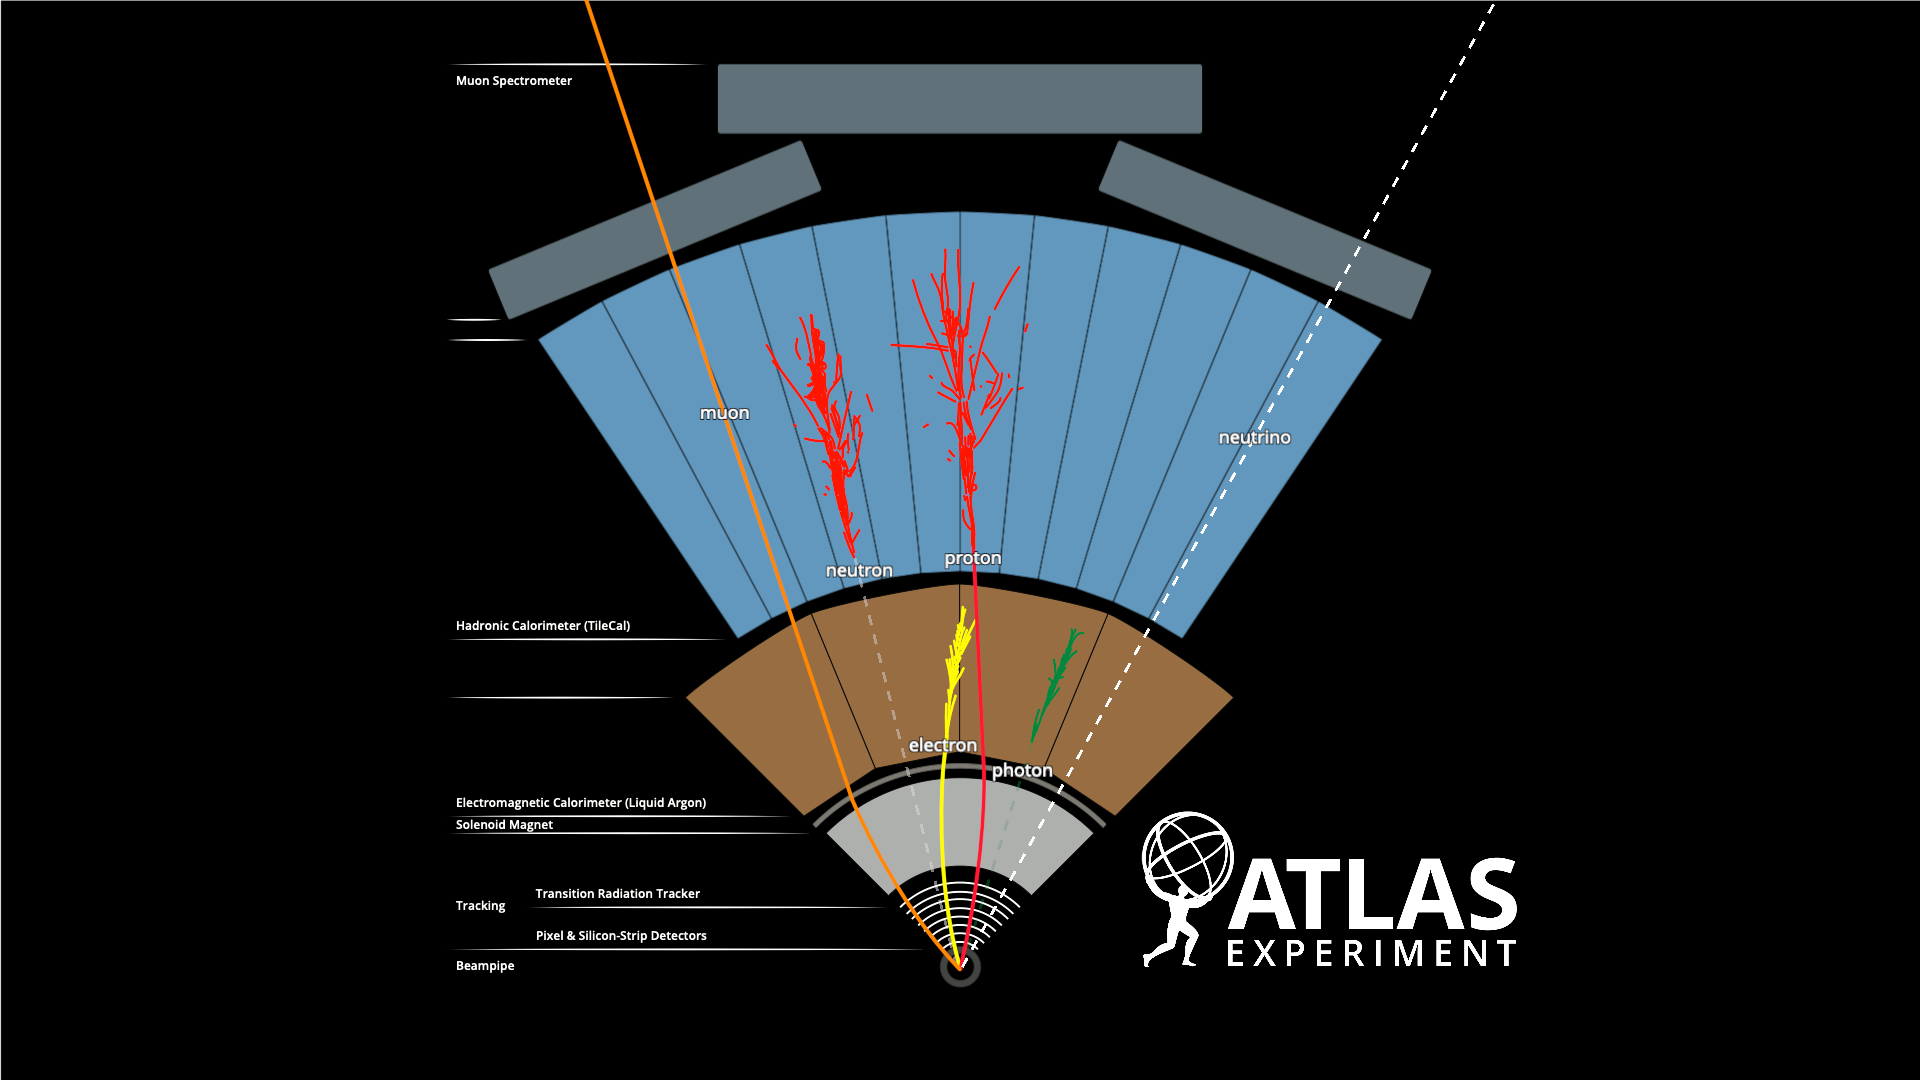
\includegraphics[width=\linewidth]{Figures/atlas/ATLAS Detector Schematic black particles.png}
    \caption{Figure describing how particles are detected at ATLAS, fetched from \href{https://cds.cern.ch/record/2770815}{	ATLAS detector slice (and particle visualisations)}, by Sascha Mehlhase \cite{Mehlhase:2770815} . }
    \label{fig:atlas_particle_detect}
\end{figure}

The features used in this analysis are computed with or fetched from the features from the detector itself. Such features includes the momentum, energy, angles etc, 
all of which are either directly measured or computed baesd on the measurements in the detector. In figure \ref{fig:atlas_particle_detect} a visualization shows how
different particles move through the detector and where they are detected. For example, energy deposits are measured using calorimeters, and the different particles 
have calorimeters specially designed for them. . \par

The ATLAS detector three selection stages before the data is stored. In order to reach the highest intensity of collisions, the LHC accellerates
packets of around $10^{11}$ protons, and collides them at a rate of 25 nanoseconds, yeilding a collision rate of 40 MHz\cite{Wang:2707056}. \cite{Bernius:2707054}

\subsubsection*{Triggers}


\subsubsection*{Data preparation}


\begin{figure}[h!]
    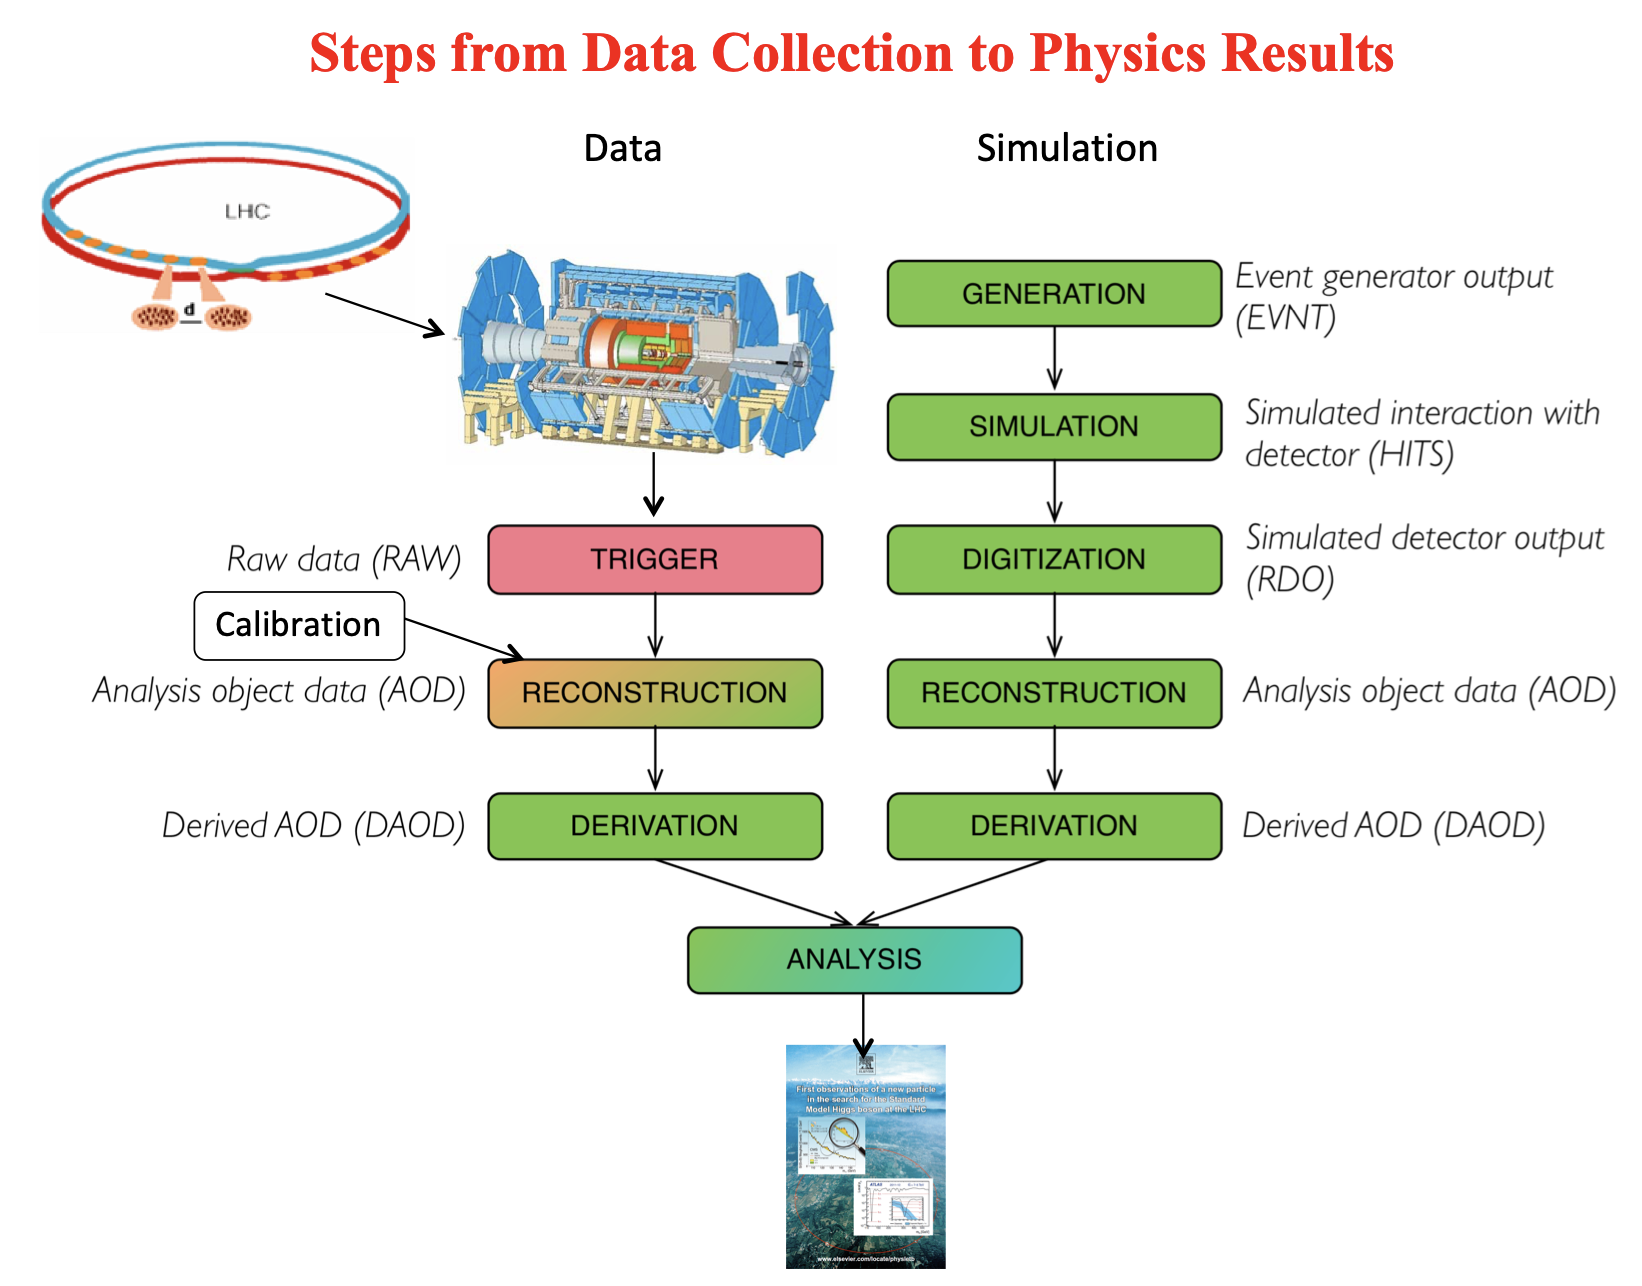
\includegraphics[width=\linewidth]{Figures/atlas/data_col_phys.png}
    \caption{Figure describing the steps to take for data collection at ATLAS, fetched from \href{https://indico.cern.ch/event/1159574/timetable/?view=standard}{Hybrid ATLAS Induction Day + Software Tutorial workshop}, part
    \href{https://indico.cern.ch/event/860971/contributions/3672974/attachments/1972049/3280896/Atlas_computing_data_preparation_jan20.pdf}{Computing and Data preparation}, 
    held by S.M Wang \cite{Wang:2707056} . }
    \label{fig:atlas_data_col_phys}
\end{figure}


\subsubsection*{Jets}
Photons and leptons are detected via calorimeters, and are easy to track and detect as they separate easily. Quarks, however, are bound by QCD and thus cannot be seperated as individual particles. 
An illustration of how quarks and gluons are behaving during a proton-proton collision is shown below in figure \ref{fig:cms_jets}.

\begin{figure}[h!]
    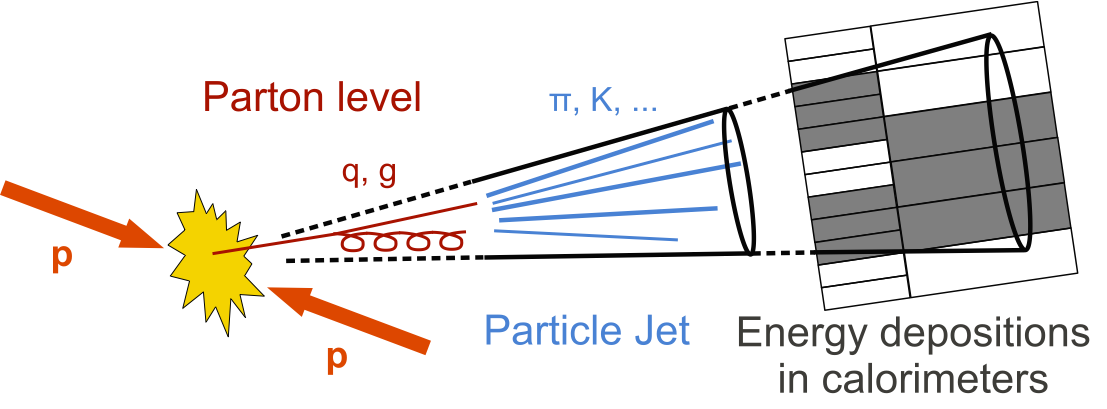
\includegraphics[width=\linewidth]{Figures/atlas/cms_Sketch_PartonParticleCaloJet.png}
    \caption{Figure describing how quarks and gluons are treated in the detector, and thus why we name them jets, fetched from \href{https://cms.cern/sites/default/files/field/image/Sketch_PartonParticleCaloJet.png}{the CMS webpage}. }
    \label{fig:cms_jets}
\end{figure}

In a proton-proton collision, the quarks and gluons forms stable or unstable hadrons such that the color confinement\footnote{Add link to a source or explanation for this.} is upheld. These then 
decay to other stable hadrons that can be tracked, and these tracks are called jets. This is particularly difficult because one wants to isolate which hadrons came from  the original quark in the 
Feynman diagram. Another point to make is that some quarks are of higher interest than others. For example, the b jet, coming from a b quark, is a good indicator for certain processes, 
thus identifying suchs particles is of huge interest. 